\documentclass[12pt]{article}

\usepackage[a4paper, margin=1in]{geometry}
\usepackage{graphicx}
\usepackage[absolute, overlay]{textpos}
\usepackage{fancyhdr}
\usepackage{siunitx}
\usepackage{tikz}
\usepackage{pgfplots}
\usetikzlibrary{decorations.pathmorphing}
\usetikzlibrary{math}
\usetikzlibrary{calc}

\pgfplotsset{compat=1.18}

\pagestyle{fancy} %for footers

\newcommand{\customsubject}{}   
\newcommand{\customtitle}{}

\newcounter{questionpartcounter}                  %Setup for question part counter for a,b,c listing
\renewcommand{\thequestionpartcounter}
{\alph{questionpartcounter}}

\newcounter{questionpartpartcounter}                  %Setup for question part  partcounter for a,b,c listing
\renewcommand{\thequestionpartpartcounter}
{\roman{questionpartcounter}}

\pagestyle{fancy} %for footers
\renewcommand{\headrulewidth}{0pt}
\fancyhf{}
\fancyfoot[R]{\thepage}

\newenvironment{worksheet}[2]
{
    
    \global\renewcommand{\customtitle}{#1}
    \global\renewcommand{\customsubject}{#2}


    \begin{textblock*}{5cm}(0.4cm,0.4cm)
   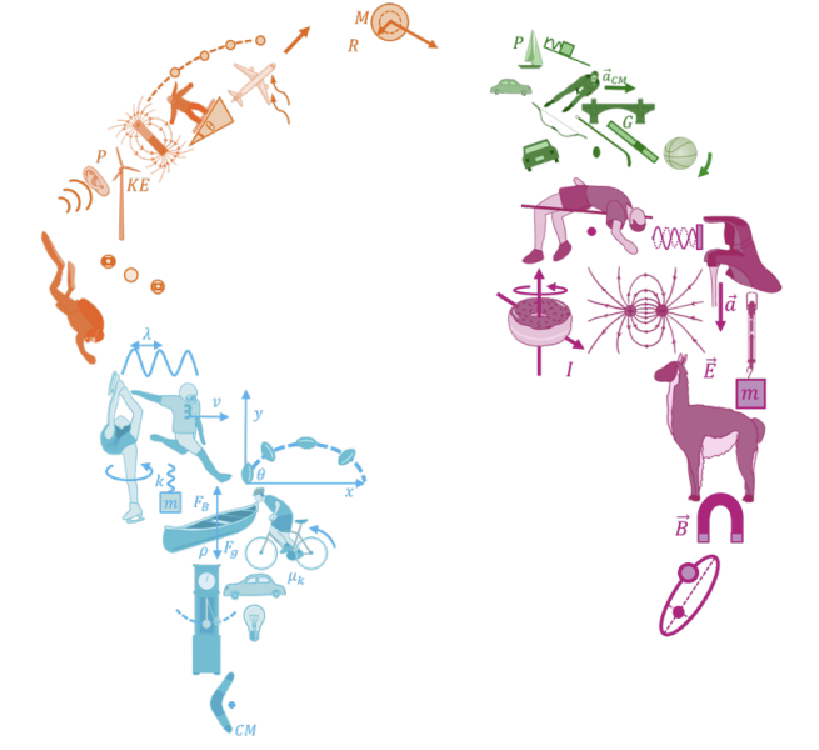
\includegraphics[width=4cm]{include/figures/bmdwlogo}
\end{textblock*}

    \vspace*{-1cm}
    
    {\large\textbf{\begin{center}\customtitle\end{center}}}

    \begin{center}\customsubject\end{center}
    
    \vspace{0.3cm}
    
    \hspace*{-1.5cm}\textbf{Name:\ \rule{4cm}{0.4pt}}\; 
    \textbf{Student \#: \ \rule{3cm}{0.4pt}}\;
    \textbf{Student Email \#: \ \rule{1.53cm}{0.4pt}}

    \vspace{0.5cm}

    
    \begin{enumerate}
}
{
    \end{enumerate}
   % \begin{textblock*}{10cm}(1cm, 28cm) {\footnotesize \scriptsize \customsubject}
    
%\end{textblock*}
}



\newcommand{\question}[2][1cm]{%
    \item
    \setcounter{questionpartcounter}{0}
    \setcounter{questionpartpartcounter}{0}
    {#2}
    \vspace{#1}
}

\newcommand{\questionpart}[2][1cm]{%
    \setcounter{questionpartpartcounter}{0}
    \stepcounter{questionpartcounter}
    (\thequestionpartcounter)~#2
    \vspace{#1}
}

\newcommand{\questionpartpart}[2][1cm]{%
      \stepcounter{questionpartpartcounter}
      \thequestionpartpartcounter.~#2
      \vspace{#1}
}

\newcommand{\operation}[1]{%
{\large $
#1
$}
}



\begin{document}

\begin{worksheet}{Physics Worksheet}{Work and Energy}

\question[4cm]{Would gravity do more et work on you if you were to drive or fly from Ottowa to Kingston?} 


\question[5cm]{Aki is a high jumper. She has a mass of 70kg. She is attempting to clear a $\SI{2}{\meter}$ high bar. Her muscles exert $\SI{2400}{\joule}$ of energy and are $50\%$ efficient at converting this into her jump. Does she clear the bar?}




\question[0cm]{Two cars ($a$ and $b$) with identical weight $m$ drive for the same amount of time $t$ from rest. Car $b$ has an engine that is 4 times more powerful than car $a$'s. What are the final velocities of the two cars?}


\newpage

\question[0.5cm]{Below, a moterized cart travels across a road. The road has a coffiecient of friction of $\mu = 0.5$. $\theta_1 = 30^\circ$ and $\theta_2 = 45^\circ$. The cart weighs $\SI{100}{\kilogram}$}

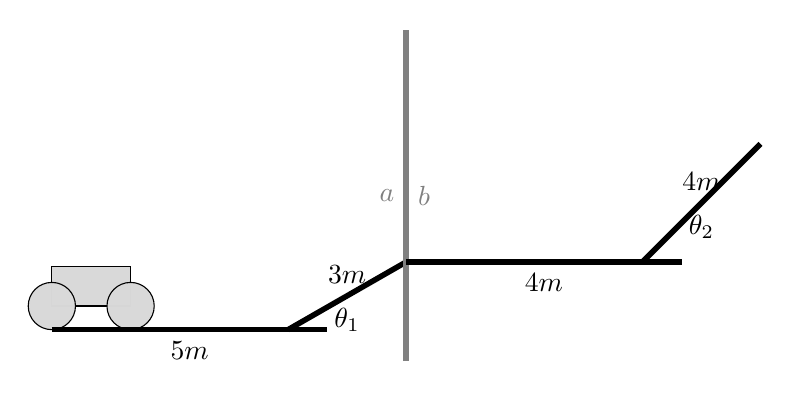
\begin{tikzpicture}

\draw[fill=gray!30] (0,-1.5) rectangle (1,-1);

\draw[fill=gray!30, fill opacity=0.99] (0.0,-1.5) circle (0.3cm);
\draw[fill=gray!30, fill opacity=0.99] (1,-1.5) circle (0.3cm);

\draw[line width = 2pt, color = black] (0.0,-1.8)--(3.5,-1.8)  node[midway, below]{$5m$};

\draw[line width = 2pt, color = black] (3,-1.8)--(4.5,-0.94)  node[midway, above]{$3m$} node[pos=0.5, below]{$\theta_1$};

\draw[line width = 2pt, color = gray] (4.5,-2.2)--(4.5,2) node[midway, left]{$a$} node[midway, right]{$b$};

\draw[line width = 2pt, color = black] (4.5,-0.94)--(8,-0.94)  node[midway, below]{$4m$};

\draw[line width = 2pt, color = black] (7.5,-0.94)--(9,0.56)  node[midway, above]{$4m$} node[pos=0.5, below]{$\theta_2$};


\end{tikzpicture}

\questionpart[6cm]{Does the friction force do more work in part $a$ or $b$ of the road?}

\questionpart[5cm]{How much work does gravity do in part $a$ and $b$?}

\questionpart[0cm]{If it takes the cart $\SI{5}{\second}$ to complete part $a$, and  $\SI{7}{\second}$ to complete part $b$, which part required the cart's motor to exert more power?}

\end{worksheet}

\end{document}